\documentclass[aspectratio=169,12pt,t]{beamer}

% --- Theme: Metropolis (modern, clean) ---
\usetheme[progressbar=frametitle,numbering=fraction,block=fill]{metropolis}

% --- Fira Sans font (install texlive-fonts-extra if missing) ---
\IfFileExists{FiraSans.sty}{\usepackage[sfdefault]{FiraSans}}{}

% --- Light background with warm accent ---
\definecolor{mDarkTeal}{RGB}{35,55,59}
\definecolor{mLightBrown}{RGB}{235,228,216}
\definecolor{mAccent}{RGB}{140,70,20}

\setbeamercolor{normal text}{fg=mDarkTeal,bg=white}
\setbeamercolor{alerted text}{fg=mAccent}
\setbeamercolor{frametitle}{bg=mDarkTeal,fg=white}
\setbeamercolor{progress bar}{fg=mAccent,bg=mLightBrown}
\setbeamercolor{title separator}{fg=mAccent}
\setbeamercolor{progress bar in head/foot}{fg=mAccent,bg=mLightBrown}
\setbeamercolor{progress bar in section page}{fg=mAccent,bg=mLightBrown}

% --- Packages ---
\usepackage[utf8]{inputenc}
\usepackage{amsmath,amssymb,amsthm}
\usepackage{mathrsfs}
\usepackage{tikz}
\usetikzlibrary{arrows.meta,positioning,calc,decorations.pathreplacing,shapes,patterns}
\usetikzlibrary{shadows.blur,backgrounds,fadings}
\usepackage{pgfplots}
\pgfplotsset{compat=1.18}

% --- Shared diagram styling (consistent, polished look across all figures) ---
\tikzset{
  axisln/.style={-{Stealth[length=2.6mm]}, line width=0.8pt, gray!75},
  curveln/.style={line width=1.6pt, line cap=round, line join=round},
  projln/.style={dash pattern=on 2.6pt off 2pt, line width=0.7pt},
  guide/.style={-{Stealth[length=2.6mm,width=2.2mm]}, line width=1.1pt},
}
% soft rounded background panel for inset plots
\tikzset{panel/.style={rounded corners=6pt, draw=mDarkTeal!14, line width=0.8pt,
  fill=mDarkTeal!4,
  blur shadow={shadow blur steps=8, shadow opacity=13,
               shadow xshift=0pt, shadow yshift=-1.3pt}}}
% point marker with a white halo: \dotpt{color}{(coord)}
\newcommand{\dotpt}[2]{%
  \fill[white] #2 circle (3.6pt);
  \fill[#1] #2 circle (2.4pt);
}
% open point marker: \opendot{color}{(coord)}
\newcommand{\opendot}[2]{%
  \fill[white] #2 circle (3.6pt);
  \draw[#1, line width=1.2pt] #2 circle (2.6pt);
}

% --- Semi-transparent white highlight for text on top of background images ---
\usepackage[most]{tcolorbox}

% Inline highlight: \hl{short text}
\newtcbox{\hl}{%
  nobeforeafter, tcbox raise base,
  colback=white, opacityback=0.6,
  colframe=white, opacityframe=0,
  sharp corners, boxsep=2pt, left=3pt, right=3pt, top=2pt, bottom=2pt%
}

% Block highlight: \begin{hlbox} ... \end{hlbox}  (multi-line, paragraphs, itemize)
\newtcolorbox{hlbox}[1][]{%
  enhanced, breakable,
  colback=white, opacityback=0.6,
  colframe=white, opacityframe=0,
  boxsep=3pt, left=6pt, right=6pt, top=4pt, bottom=4pt,
  sharp corners,
  {#1}%
}

% --- Custom colors for content types ---
\definecolor{defcolor}{RGB}{25,85,120}
\definecolor{thmcolor}{RGB}{140,35,35}
\definecolor{proofcolor}{RGB}{35,100,50}
\definecolor{excolor}{RGB}{140,75,10}
\definecolor{remcolor}{RGB}{90,90,90}

% --- Beamer blocks for mathematical content types (semi-transparent) ---
\tcbset{hlblockbase/.style={
  enhanced, breakable,
  coltitle=white, fonttitle=\bfseries,
  opacitybacktitle=0.8, opacityback=0.6,
  opacityframe=0,
  sharp corners,
  boxsep=1pt, left=5pt, right=5pt, top=2pt, bottom=2pt,
  toptitle=1pt, bottomtitle=1pt
}}

\newtcolorbox{defblock}[1]{hlblockbase, title={#1},
  colbacktitle=defcolor, colback=defcolor!15, colframe=defcolor}
\newtcolorbox{thmblock}[1]{hlblockbase, title={#1},
  colbacktitle=thmcolor, colback=thmcolor!15, colframe=thmcolor}
\newtcolorbox{proofblock}[1]{hlblockbase, title={#1},
  colbacktitle=proofcolor, colback=proofcolor!15, colframe=proofcolor}
\newtcolorbox{exblock}[1]{hlblockbase, title={#1},
  colbacktitle=excolor, colback=excolor!15, colframe=excolor}
\newtcolorbox{remblock}[1]{hlblockbase, title={#1},
  colbacktitle=remcolor, colback=remcolor!15, colframe=remcolor}

% --- Metadata ---
\title{Chapter 5: Differentiation}
\subtitle{Section: The Derivative of a Real Function}
\author{Based on Walter Rudin's \emph{Principles of Mathematical Analysis}}
\date{}

\begin{document}

{
\usebackgroundtemplate{%
  
\includegraphics[width=\paperwidth,height=\paperheight,keepaspectratio=false]{chapter_05_bg_00.png}%
}
\begin{frame}[plain]
  \titlepage
  \note{
    Welcome to Chapter 5, which is all about differentiation. In this first
    section we define the derivative of a real function, prove that
    differentiability implies continuity, establish the rules for
    differentiating sums, products, quotients, and compositions, and finish
    with two famous examples that reveal how subtle derivatives can be.
    Throughout this chapter we work with real functions defined on intervals.
    This restriction is deliberate, since genuinely new phenomena appear for
    vector valued functions, and those will wait until the last section of the
    chapter and until Chapter 9. Let's get started.
  }
\end{frame}
}

{
\usebackgroundtemplate{%
  
\includegraphics[width=\paperwidth,height=\paperheight,keepaspectratio=false]{chapter_05_bg_01.png}%
}
\begin{frame}[c]{Outline}
  \begin{center}
    \tableofcontents
  \end{center}
  \note{
    Here is our roadmap. We start with some motivation, then give the precise
    definition of the derivative as a limit of difference quotients. Next we
    prove that differentiability implies continuity, and we develop the
    algebra of derivatives, the sum, product, and quotient rules. After that
    comes the chain rule, probably the most important theorem about
    derivatives. We end with two instructive examples built from oscillating
    functions, and a summary that points ahead to the mean value theorems.
  }
\end{frame}

\section{Motivation}

% --- Build 1/3 ---
\begin{frame}{Why This Section Matters}
  \begin{hlbox}
  \begin{itemize}
    \item Chapter 4 studied \emph{continuity}: how $f(t)$ behaves as $t \to x$
  \end{itemize}
  \end{hlbox}

  \note{
    Let's put this section in context. In Chapter 4 we studied continuity,
    which asks a qualitative question: does "f" of "t" approach "f" of "x"
    as "t" approaches "x"? Continuity tells us that a function has no sudden
    jumps, but it says nothing about how fast the function changes.
  }
\end{frame}

% --- Build 2/3 ---
\begin{frame}{Why This Section Matters}
  \begin{hlbox}
  \begin{itemize}
    \item Chapter 4 studied \emph{continuity}: how $f(t)$ behaves as $t \to x$
    \item The derivative asks a sharper question: the \alert{rate of change}
      \[
        \frac{f(t) - f(x)}{t - x} \quad \text{as } t \to x
      \]
  \end{itemize}
  \end{hlbox}

  \note{
    The derivative asks a sharper, quantitative question. Instead of just
    watching "f" of "t" approach "f" of "x", we compare the change in the
    function to the change in the input. That ratio, shown on the slide, is
    the average rate of change between "x" and "t". The derivative is what
    happens to this ratio in the limit, and notice that this is exactly the
    kind of function limit we defined in Chapter 4. Everything we learned
    about limits is about to pay off.
  }
\end{frame}

% --- Build 3/3 ---
\begin{frame}{Why This Section Matters}
  \begin{hlbox}
  \begin{itemize}
    \item Chapter 4 studied \emph{continuity}: how $f(t)$ behaves as $t \to x$
    \item The derivative asks a sharper question: the \alert{rate of change}
      \[
        \frac{f(t) - f(x)}{t - x} \quad \text{as } t \to x
      \]
    \item Preview: differentiable $\Rightarrow$ continuous, algebraic rules,
      the \alert{chain rule}, and two surprising examples
  \end{itemize}
  \end{hlbox}

  \note{
    Here is what we will accomplish. First, differentiability is stronger
    than continuity: every differentiable function is continuous, but not
    conversely. Second, derivatives interact nicely with sums, products, and
    quotients, so all polynomials and rational functions are differentiable.
    Third, the chain rule handles compositions. And finally, two examples
    with oscillating functions will show that a derivative can exist
    everywhere yet fail to be continuous. Let's begin with the definition.
  }
\end{frame}
}

{
\usebackgroundtemplate{%
  
\includegraphics[width=\paperwidth,height=\paperheight,keepaspectratio=false]{chapter_05_bg_02.png}%
}
\section{Definition of the Derivative}

\begin{frame}{The Geometric Picture: Secants Becoming Tangents}
  \begin{center}
  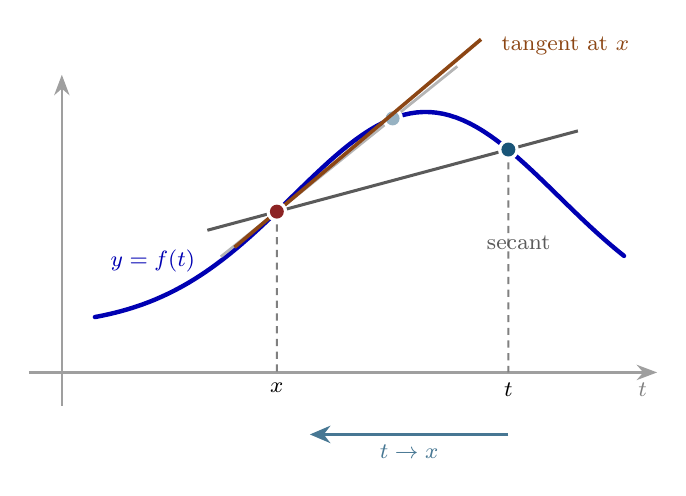
\begin{tikzpicture}[scale=1.05]
    % Axes
    \draw[axisln] (-0.4,0) -- (7.2,0) node[below left, gray]{\footnotesize $t$};
    \draw[axisln] (0,-0.4) -- (0,3.6);
    % Curve f
    \draw[curveln, blue!70!black, domain=0.4:6.8, samples=80]
      plot (\x, {0.55 + 2.6*exp(-0.5*(\x-4.4)*(\x-4.4)/2.6)});
    \node[blue!70!black] at (1.1,1.35) {\footnotesize $y = f(t)$};
    % Points x and t
    \coordinate (P) at (2.6, {0.55 + 2.6*exp(-0.5*(2.6-4.4)*(2.6-4.4)/2.6)});
    \coordinate (Q) at (5.4, {0.55 + 2.6*exp(-0.5*(5.4-4.4)*(5.4-4.4)/2.6)});
    % Fainter secant: t has moved closer to x
    \coordinate (Q2) at (4.0, {0.55 + 2.6*exp(-0.5*(4.0-4.4)*(4.0-4.4)/2.6)});
    \draw[remcolor!45, line width=1.0pt, shorten <=-26pt, shorten >=-30pt] (P) -- (Q2);
    \dotpt{defcolor!45}{(Q2)}
    % Secant line through P and Q
    \draw[remcolor, line width=1.1pt, shorten <=-26pt, shorten >=-26pt] (P) -- (Q);
    % Tangent line at P (approximate slope)
    \draw[mAccent, line width=1.3pt, shorten <=-20pt, shorten >=-34pt]
      (P) -- ($(P)+(1.6,1.35)$);
    % Projections
    \draw[projln, gray] (P) -- (2.6,0) node[below, black]{\footnotesize $x$};
    \draw[projln, gray] (Q) -- (5.4,0) node[below, black]{\footnotesize $t$};
    \dotpt{thmcolor}{(P)}
    \dotpt{defcolor}{(Q)}
    \node[remcolor, above right=1pt] at (5.0,1.35) {\footnotesize secant};
    \node[mAccent, right] at (5.2,3.95) {\footnotesize tangent at $x$};
    % Arrow: t moves toward x
    \draw[guide, defcolor!80] (5.4,-0.75) -- (3.0,-0.75)
      node[midway, below]{\footnotesize $t \to x$};
  \end{tikzpicture}
  \end{center}

  \note{
    Before the formal definition, here is the picture to keep in mind. The
    blue curve is the graph of a function "f". We fix the red point above
    "x" and pick a second, blue point above "t". The gray line through the
    two points is a secant line, and its slope is exactly the difference
    quotient, the change in "f" divided by the change in the input. Now
    slide "t" toward "x", as the arrow at the bottom indicates. The fainter
    gray line shows the secant after "t" has moved closer: the blue point
    travels along the curve toward the red point, and the secants tilt
    toward the orange line, the tangent at "x". The derivative, if it
    exists, is the slope of that tangent line. Let's now say this precisely.
  }
\end{frame}

% --- Build 1/2 ---
\begin{frame}{Definition 5.1: The Derivative}
  \begin{defblock}{Definition 5.1 (part 1: the difference quotient)}
    Let $f$ be real-valued on $[a,b]$. For $x \in [a,b]$ form
    \begin{equation}
      \phi(t) = \frac{f(t) - f(x)}{t - x} \qquad (a < t < b,\; t \neq x) \tag{1}
    \end{equation}
  \end{defblock}

  \note{
    Here is the formal setup. We take a real valued function "f" defined on
    the closed interval from "a" to "b", and we fix a point "x" in that
    interval. For every other point "t" we form the quotient phi of "t"
    shown in equation 1: the difference of the function values divided by
    the difference of the inputs. Geometrically this is the slope of the
    secant line we just saw. Note that "t" ranges over the interval but must
    stay different from "x", so the quotient is always well defined. Next we
    take the limit.
  }
\end{frame}

% --- Build 2/2 ---
\begin{frame}{Definition 5.1: The Derivative}
  \begin{defblock}{Definition 5.1 (part 1: the difference quotient)}
    Let $f$ be real-valued on $[a,b]$. For $x \in [a,b]$ form
    \begin{equation}
      \phi(t) = \frac{f(t) - f(x)}{t - x} \qquad (a < t < b,\; t \neq x) \tag{1}
    \end{equation}
  \end{defblock}

  \begin{defblock}{Definition 5.1 (part 2: the derivative)}
    \begin{equation}
      f'(x) = \lim_{t \to x} \phi(t), \tag{2}
    \end{equation}
    provided this limit exists (in the sense of Definition 4.1).
  \end{defblock}

  \note{
    The derivative of "f" at "x", written "f" prime of "x", is the limit of
    the difference quotient as "t" tends to "x", equation 2 on the slide.
    The crucial phrase is: provided this limit exists. This is exactly the
    limit concept of Definition 4.1 from the previous chapter, applied to
    the function phi. So the derivative is not a new kind of limit; it is
    our old friend, the limit of a function, applied to a cleverly chosen
    auxiliary function. Of course, the limit may fail to exist, and that is
    where the interesting examples live.
  }
\end{frame}

\begin{frame}{Differentiable Functions}
  \begin{defblock}{Terminology}
    \begin{itemize}
      \item $f'$ is the \alert{derivative} of $f$; its domain is the set of
        points $x$ where the limit (2) exists
      \item If $f'(x)$ is defined, $f$ is \alert{differentiable at $x$}
      \item If $f'$ is defined at every point of $E \subset [a,b]$,\\
        then $f$ is \alert{differentiable on $E$}
    \end{itemize}
  \end{defblock}

  \note{
    This definition attaches to the function "f" a brand new function,
    "f" prime, called the derivative of "f". Its domain consists of all
    points "x" where the limit in equation 2 exists; there is no guarantee
    that this is the whole interval. When "f" prime is defined at a specific
    point "x", we say that "f" is differentiable at "x". And when "f" prime
    is defined at every point of a subset "E" of the interval, we say "f"
    is differentiable on "E". Keep in mind this view of the derivative as a
    function in its own right; the question of whether "f" prime is itself
    continuous will return at the end of this section. Before our first
    theorem, a few words about endpoints.
  }
\end{frame}

\begin{frame}{One-Sided Derivatives and Endpoints}
  \begin{remblock}{Remarks on the domain}
    \begin{itemize}
      \item Right-hand / left-hand limits in (2) give \emph{one-sided}
        derivatives
      \item At the endpoints $a$ and $b$, the derivative is a
        one-sided derivative
      \item If $f$ is defined only on a segment $(a,b)$, then $f'(a)$, $f'(b)$
        are \alert{not defined}
    \end{itemize}
  \end{remblock}

  \note{
    A few remarks about the edges of the interval. If we use a right-hand
    or a left-hand limit in equation 2, we get one-sided derivatives. In
    particular, at the left endpoint "a" the only available derivative is a
    right-hand one, and at "b" a left-hand one. Rudin mentions these but
    does not develop one-sided derivatives in any detail, and neither will
    we. Finally, if "f" lives only on the open segment from "a" to "b",
    then the derivative is defined by the same two equations at interior
    points, but the derivative at the endpoints simply does not exist,
    because the function is not defined there. With the definition settled,
    let's prove our first theorem.
  }
\end{frame}
}

{
\usebackgroundtemplate{%
  
\includegraphics[width=\paperwidth,height=\paperheight,keepaspectratio=false]{chapter_05_bg_03.png}%
}
\section{Differentiability Implies Continuity}

\begin{frame}{Theorem 5.2: Differentiable $\Rightarrow$ Continuous}
  \begin{thmblock}{Theorem 5.2}
    Let $f$ be defined on $[a,b]$. If $f$ is differentiable at a point
    $x \in [a,b]$, then $f$ is continuous at $x$.
  \end{thmblock}

  \vspace{0.5em}
  \begin{hlbox}
  \textbf{Key idea:} differentiability is a \alert{stronger} condition than
  continuity.
  \end{hlbox}

  \note{
    Our first theorem connects the new concept to the old one. If "f" is
    differentiable at a point "x", then "f" is automatically continuous at
    that point. In other words, differentiability is a strictly stronger
    requirement than continuity: asking for the difference quotient to have
    a limit forces the function values themselves to converge. The proof is
    a one-line trick, but a very instructive one. Let's see it.
  }
\end{frame}

\begin{frame}{Proof of Theorem 5.2}
  \begin{proofblock}{Proof: multiply and divide by $t - x$}
    As $t \to x$, by Theorem 4.4 (algebra of limits),
    \[
      f(t) - f(x) = \underbrace{\frac{f(t) - f(x)}{t - x}}_{\to\; f'(x)}
        \cdot \underbrace{(t - x)}_{\to\; 0}
        \;\longrightarrow\; f'(x) \cdot 0 = 0. \qquad \blacksquare
    \]
  \end{proofblock}

  \vspace{0.5em}
  \begin{hlbox}
  \textbf{Technique:} rewrite a difference as \emph{quotient} $\times$
  \emph{increment}, then apply the algebra of limits.
  \end{hlbox}

  \note{
    Here is the whole proof in one line. We want to show that "f" of "t"
    minus "f" of "x" tends to zero. The trick is to multiply and divide by
    "t" minus "x", as shown on the slide. The first factor is the difference
    quotient, which tends to "f" prime of "x" because "f" is differentiable
    at "x". The second factor, "t" minus "x", obviously tends to zero. By
    Theorem 4.4, the limit of a product is the product of the limits, so the
    whole expression tends to "f" prime of "x" times zero, which is zero.
    That is precisely continuity at "x". Remember this technique of writing
    a difference as quotient times increment; it reappears constantly.
    Now, what about the converse?
  }
\end{frame}

\begin{frame}{The Converse Fails}
  \begin{remblock}{Warning: continuity does \emph{not} imply differentiability}
    \begin{itemize}
      \item Continuous functions can fail to be differentiable at isolated
        points
      \item Chapter 7: a function continuous on \alert{all} of $\mathbb{R}$,
        differentiable \alert{nowhere}!
    \end{itemize}
  \end{remblock}

  \begin{center}
  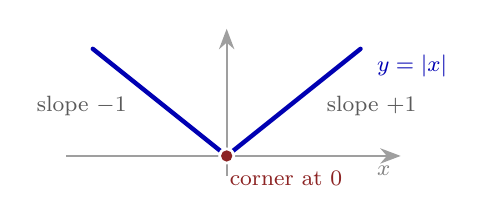
\begin{tikzpicture}[scale=0.85]
    \draw[axisln] (-2.4,0) -- (2.6,0) node[below left, gray]{\footnotesize $x$};
    \draw[axisln] (0,-0.3) -- (0,1.9);
    \draw[curveln, blue!70!black] (-2.0,1.6) -- (0,0) -- (2.0,1.6);
    \dotpt{thmcolor}{(0,0)}
    \node[blue!70!black, right] at (2.1,1.35) {\footnotesize $y = |x|$};
    \node[thmcolor, below right] at (-0.1,-0.08) {\footnotesize corner at $0$};
    \node[remcolor, anchor=east] at (-1.35,0.75) {\footnotesize slope $-1$};
    \node[remcolor, anchor=west] at (1.35,0.75) {\footnotesize slope $+1$};
  \end{tikzpicture}
  \end{center}

  \note{
    Does continuity imply differentiability? Not at all.
    The picture shows the standard counterexample: the absolute value
    function. It is continuous everywhere, but at zero the graph has a
    corner, marked by the red dot. As the labels indicate, secant slopes
    from the right equal plus one while secant slopes from the left equal
    minus one, so the limit of the difference quotient does not exist
    there. Failure at isolated points
    is easy to arrange. But it gets far more dramatic: in Chapter 7 we will
    meet a function that is continuous at every real number yet
    differentiable at none of them. Continuity is a much weaker property
    than the smooth pictures suggest. Now let's build up the algebra of
    derivatives.
  }
\end{frame}
}

{
\usebackgroundtemplate{%
  
\includegraphics[width=\paperwidth,height=\paperheight,keepaspectratio=false]{chapter_05_bg_04.png}%
}
\section{Algebra of Derivatives}

% --- Build 1/3 ---
\begin{frame}{Theorem 5.3: Sum, Product, and Quotient Rules}
  \begin{thmblock}{Theorem 5.3}
    Suppose $f$, $g$ are defined on $[a,b]$ and differentiable at
    $x \in [a,b]$. Then $f+g$, $fg$, $f/g$ are differentiable at $x$, and
    \begin{enumerate}
      \item[(a)] $(f+g)'(x) = f'(x) + g'(x)$
    \end{enumerate}
  \end{thmblock}

  \note{
    Next, the arithmetic of derivatives. We take two functions, "f" and
    "g", both differentiable at the same point "x". The theorem says that
    their sum, their product, and their quotient are then differentiable at
    "x" as well, and it gives explicit formulas. Part "a" is the simplest:
    the derivative of a sum is the sum of the derivatives. This follows
    immediately from Theorem 4.4, since the difference quotient of "f" plus
    "g" splits into the difference quotient of "f" plus that of "g". The
    product rule is more interesting.
  }
\end{frame}

% --- Build 2/3 ---
\begin{frame}{Theorem 5.3: Sum, Product, and Quotient Rules}
  \begin{thmblock}{Theorem 5.3}
    Suppose $f$, $g$ are defined on $[a,b]$ and differentiable at
    $x \in [a,b]$. Then $f+g$, $fg$, $f/g$ are differentiable at $x$, and
    \begin{enumerate}
      \item[(a)] $(f+g)'(x) = f'(x) + g'(x)$
      \item[(b)] $(fg)'(x) = f'(x)g(x) + f(x)g'(x)$
    \end{enumerate}
  \end{thmblock}

  \note{
    Part "b" is the product rule: the derivative of the product is the
    derivative of the first times the second, plus the first times the
    derivative of the second. Notice the structure: each factor gets
    differentiated exactly once, while the other is left alone. This
    asymmetric looking formula is forced by the way increments of a product
    decompose, as we will see in the proof in a moment. Finally, the
    quotient rule.
  }
\end{frame}

% --- Build 3/3 ---
\begin{frame}{Theorem 5.3: Sum, Product, and Quotient Rules}
  \begin{thmblock}{Theorem 5.3}
    Suppose $f$, $g$ are defined on $[a,b]$ and differentiable at
    $x \in [a,b]$. Then $f+g$, $fg$, $f/g$ are differentiable at $x$, and
    \begin{enumerate}
      \item[(a)] $(f+g)'(x) = f'(x) + g'(x)$
      \item[(b)] $(fg)'(x) = f'(x)g(x) + f(x)g'(x)$
      \item[(c)] $\displaystyle\left(\frac{f}{g}\right)'(x)
        = \frac{g(x)f'(x) - g'(x)f(x)}{g^2(x)}$
        \quad (assuming $g(x) \neq 0$)
    \end{enumerate}
  \end{thmblock}

  \note{
    Part "c" is the quotient rule: the derivative of "f" over "g" is "g"
    times "f" prime minus "g" prime times "f", all divided by "g" squared.
    For this to make sense we naturally assume that "g" of "x" is not zero;
    then continuity of "g", which we just proved in Theorem 5.2, keeps "g"
    of "t" away from zero for "t" near "x". Together, these three rules
    say that differentiable functions form an algebra, closed under the
    usual operations. Let's prove parts "b" and "c".
  }
\end{frame}

\begin{frame}{Proof of Theorem 5.3(b): The Product Rule}
  \begin{proofblock}{Proof of (b): split the increment of $h = fg$}
    \[
      h(t) - h(x) = f(t)\bigl[g(t) - g(x)\bigr] + g(x)\bigl[f(t) - f(x)\bigr]
    \]
    Divide by $t - x$; as $t \to x$, use $f(t) \to f(x)$ (Theorem 5.2):
    \begin{align*}
      \frac{h(t)-h(x)}{t-x}
      &= f(t)\,\frac{g(t)-g(x)}{t-x} + g(x)\,\frac{f(t)-f(x)}{t-x} \\
      &\to\; f(x)g'(x) + g(x)f'(x). \qquad \blacksquare
    \end{align*}
  \end{proofblock}

  \note{
    For the product rule, let "h" be the product of "f" and "g". The first
    line on the slide is the key algebraic identity: the increment of the
    product is split by adding and subtracting the cross term "f" of "t"
    times "g" of "x". Check it by expanding; everything cancels perfectly.
    Now divide by "t" minus "x". Each bracket becomes a difference quotient,
    as in the second line. As "t" tends to "x", the difference quotients
    tend to "g" prime of "x" and "f" prime of "x" respectively, and the
    factor "f" of "t" tends to "f" of "x" precisely because differentiable
    functions are continuous; this is where Theorem 5.2 earns its keep. The
    limit is "f" of "x" times "g" prime of "x" plus "g" of "x" times "f"
    prime of "x", which is the product rule.
  }
\end{frame}

\begin{frame}{Proof of Theorem 5.3(c): The Quotient Rule}
  \begin{proofblock}{Proof of (c): same idea for $h = f/g$}
    \begin{small}
    \[
      \frac{h(t) - h(x)}{t - x}
      = \frac{1}{g(t)g(x)}
        \left[ g(x)\frac{f(t)-f(x)}{t-x} - f(x)\frac{g(t)-g(x)}{t-x} \right]
    \]
    \end{small}
    Let $t \to x$: by Theorems 4.4 and 5.2,
    \[
      h'(x) = \frac{g(x)f'(x) - g'(x)f(x)}{g^2(x)}. \qquad \blacksquare
    \]
  \end{proofblock}

  \note{
    The quotient rule follows the same pattern. Let "h" be "f" over "g".
    A short computation, again by adding and subtracting a cross term in
    the numerator, puts the difference quotient of "h" into the form shown:
    a prefactor, one over "g" of "t" times "g" of "x", multiplying a
    combination of the difference quotients of "f" and of "g". Now let "t"
    tend to "x". By continuity, "g" of "t" tends to "g" of "x", so the
    prefactor tends to one over "g" squared. The two inner quotients tend
    to "f" prime and "g" prime, and assembling everything with Theorem 4.4
    gives exactly the quotient rule. Both proofs are just algebra plus the
    limit theorems. Let's harvest the consequences.
  }
\end{frame}

% --- Build 1/2 ---
\begin{frame}{Examples 5.4: Building a Library of Derivatives}
  \begin{exblock}{Examples 5.4}
    \begin{itemize}
      \item Constants: $f(x) = c \;\Rightarrow\; f'(x) = 0$
      \item Identity: $f(x) = x \;\Rightarrow\; f'(x) = 1$
    \end{itemize}
  \end{exblock}

  \note{
    From two trivial building blocks we can now differentiate a huge class
    of functions. First, the derivative of a constant is zero: the
    numerator of the difference quotient vanishes identically. Second, if
    "f" of "x" equals "x", the difference quotient is identically one, so
    the derivative is one everywhere. These two computations come straight
    from the definition, no theorems needed. Now the algebra of derivatives
    takes over.
  }
\end{frame}

% --- Build 2/2 ---
\begin{frame}{Examples 5.4: Building a Library of Derivatives}
  \begin{exblock}{Examples 5.4}
    \begin{itemize}
      \item Constants: $f(x) = c \;\Rightarrow\; f'(x) = 0$
      \item Identity: $f(x) = x \;\Rightarrow\; f'(x) = 1$
      \item Repeated use of (b), (c): \quad
        $\bigl(x^n\bigr)' = n x^{n-1}$ \quad (integer $n$; $x \neq 0$ if $n<0$)
      \item Hence every \alert{polynomial} is differentiable, and every
        \alert{rational function} is, except where its denominator vanishes
    \end{itemize}
  \end{exblock}

  \note{
    Applying the product rule repeatedly to "x" times "x" times "x" and so
    on shows that "x" to the "n" is differentiable with derivative "n"
    times "x" to the "n" minus one, for every positive integer "n". The
    quotient rule then extends this to negative integer exponents, as long
    as we stay away from "x" equals zero. Consequently every polynomial is
    differentiable everywhere, and every rational function, a quotient of
    polynomials, is differentiable except at the points where its
    denominator vanishes. With sums, products, and quotients under control,
    one operation remains: composition. That is the chain rule, and it
    deserves its own section.
  }
\end{frame}
}

{
\usebackgroundtemplate{%
  
\includegraphics[width=\paperwidth,height=\paperheight,keepaspectratio=false]{chapter_05_bg_05.png}%
}
\section{The Chain Rule}

\begin{frame}{Theorem 5.5: The Chain Rule}
  \begin{thmblock}{Theorem 5.5}
    Suppose $f$ is continuous on $[a,b]$, $f'(x)$ exists at some
    $x \in [a,b]$, $g$ is defined on an interval $I \supset f([a,b])$, and
    $g$ is differentiable at $f(x)$. If
    \[
      h(t) = g(f(t)) \qquad (a \leq t \leq b),
    \]
    then $h$ is differentiable at $x$, and
    \begin{equation}
      h'(x) = g'(f(x))\,f'(x). \tag{3}
    \end{equation}
  \end{thmblock}

  \note{
    Here is the chain rule, which the book describes as probably the most
    important theorem about derivatives. It tells us how to differentiate a
    composition. Read the hypotheses carefully: "f" is continuous on the
    whole interval and differentiable at the single point "x"; "g" is
    defined on an interval containing the range of "f", and "g" is
    differentiable at the point "f" of "x", the image of "x". Then the
    composite function "h", "g" after "f", is differentiable at "x", and
    equation 3 says its derivative is the product of the two derivatives:
    "g" prime evaluated at "f" of "x", times "f" prime at "x". The outer
    derivative is evaluated at the inner value; that is the detail people
    forget. More general versions await in Chapter 9.
  }
\end{frame}

\begin{frame}{Chain Rule: The Composition Picture}
  \begin{center}
  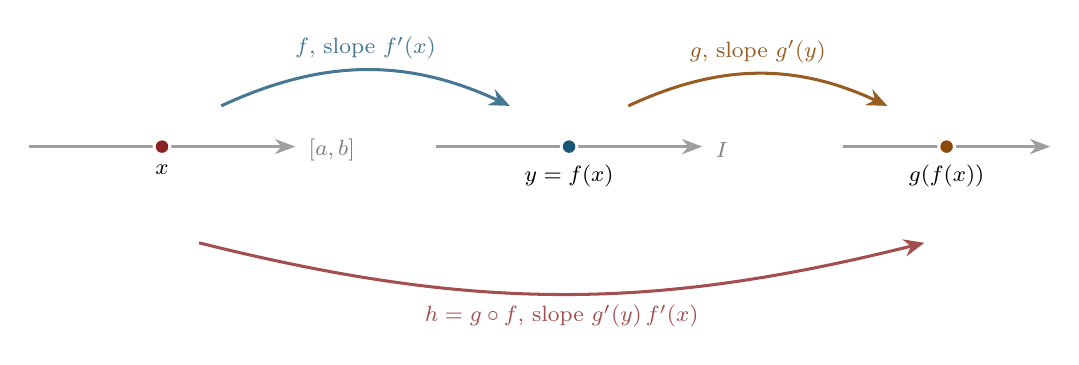
\begin{tikzpicture}[scale=0.94]
    % Domain line
    \draw[axisln] (-0.3,0) -- (3.3,0);
    \node[gray, right] at (3.35,-0.05) {\footnotesize $[a,b]$};
    \dotpt{thmcolor}{(1.5,0)}
    \node[below=3pt] at (1.5,0) {\footnotesize $x$};
    % Middle line
    \draw[axisln] (5.2,0) -- (8.8,0);
    \node[gray, right] at (8.85,-0.05) {\footnotesize $I$};
    \dotpt{defcolor}{(7.0,0)}
    \node[below=3pt] at (7.0,0) {\footnotesize $y = f(x)$};
    % Target line
    \draw[axisln] (10.7,0) -- (13.5,0);
    \dotpt{excolor}{(12.1,0)}
    \node[below=3pt] at (12.1,0) {\footnotesize $g(f(x))$};
    % Maps
    \draw[guide, defcolor!80] (2.3,0.55) to[bend left=25]
      node[midway, above]{\footnotesize $f$, slope $f'(x)$} (6.2,0.55);
    \draw[guide, excolor!90] (7.8,0.55) to[bend left=25]
      node[midway, above]{\footnotesize $g$, slope $g'(y)$} (11.3,0.55);
    \draw[guide, thmcolor!80] (2.0,-1.3) to[bend right=14]
      node[midway, below]{\footnotesize $h = g \circ f$, slope $g'(y)\,f'(x)$}
      (11.8,-1.3);
  \end{tikzpicture}
  \end{center}

  \vspace{0.1em}
  \begin{hlbox}
  \textbf{Intuition:} small increments get scaled by $f'(x)$, then by
  $g'(y)$ --- so the total scaling is the \alert{product}.
  \end{hlbox}

  \note{
    This diagram shows why the answer is a product. On the left is the
    domain of "f" with our point "x" in red. The first arrow, in blue, sends
    it through "f" to the middle line, landing at the blue point "y" equals
    "f" of "x", inside the interval "I". The second arrow, in amber, applies
    "g", landing at the amber point "g" of "f" of "x" on the right. The long red
    arrow underneath is the composite map "h". Now think of derivatives as
    local scaling factors for small increments. Near "x", the map "f"
    stretches increments by roughly "f" prime of "x". Near "y", the map "g"
    stretches them by "g" prime of "y". Doing one after the other
    multiplies the two factors, and that is exactly formula 3. The proof
    makes this rigorous with a clever linearization.
  }
\end{frame}

% --- Build 1/3 ---
\begin{frame}{Proof of Theorem 5.5}
  \begin{hlbox}
  \textbf{Strategy:} rewrite differentiability as a \alert{linear
  approximation} with a vanishing error term.
  \end{hlbox}

  \begin{proofblock}{Step 1: linearize $f$ at $x$ and $g$ at $y = f(x)$}
    \begin{align}
      f(t) - f(x) &= (t-x)\,\bigl[f'(x) + u(t)\bigr], \tag{4}\\
      g(s) - g(y) &= (s-y)\,\bigl[g'(y) + v(s)\bigr], \tag{5}
    \end{align}
    where $u(t) \to 0$ as $t \to x$, and $v(s) \to 0$ as $s \to y$.
  \end{proofblock}

  \note{
    The proof introduces a technique that will pay dividends for the rest
    of the book: replace the limit statement by an exact identity with an
    error term. Since "f" is differentiable at "x", the difference quotient
    minus "f" prime of "x" tends to zero; call that difference "u" of "t".
    Multiplying out gives equation 4: the increment of "f" equals the
    increment of the input times "f" prime of "x" plus the error "u" of
    "t", where "u" tends to zero. Equation 5 does the same for "g" at the
    point "y", with error term "v" of "s". These identities hold exactly,
    for all "t" in the interval and "s" in "I", not just in the limit. Now
    we chain them together.
  }
\end{frame}

% --- Build 2/3 ---
\begin{frame}{Proof of Theorem 5.5}
  \begin{proofblock}{Step 2: substitute $s = f(t)$ and chain the identities}
    Using first (5), then (4):
    \begin{align*}
      h(t) - h(x) &= g(f(t)) - g(f(x)) \\
      &= [f(t) - f(x)] \cdot [g'(y) + v(s)] \\
      &= (t-x) \cdot [f'(x) + u(t)] \cdot [g'(y) + v(s)]
    \end{align*}
    so for $t \neq x$:
    \begin{equation}
      \frac{h(t) - h(x)}{t - x} = [g'(y) + v(s)] \cdot [f'(x) + u(t)] \tag{6}
    \end{equation}
  \end{proofblock}

  \note{
    Step 2 is the heart of the proof. We plug "s" equals "f" of "t" into
    identity 5. The increment of "h" is "g" of "f" of "t" minus "g" of "f"
    of "x", and identity 5 turns this into the increment of "f" times the
    bracket "g" prime of "y" plus "v" of "s". Then identity 4 expands the
    increment of "f" itself, producing the third line: "t" minus "x" times
    both brackets. Dividing by "t" minus "x" for "t" different from "x"
    gives equation 6, an exact formula for the difference quotient of the
    composite. Notice how the two error terms sit harmlessly inside their
    brackets. One subtle point: this argument never divides by "f" of "t"
    minus "f" of "x", which could be zero; that is exactly the pitfall the
    linearization trick avoids.
  }
\end{frame}

% --- Build 3/3 ---
\begin{frame}{Proof of Theorem 5.5}
  \begin{proofblock}{Step 3: let $t \to x$}
    \begin{itemize}
      \item $f$ continuous at $x$ $\;\Rightarrow\;$ $s = f(t) \to y$
      \item Hence $u(t) \to 0$ and $v(s) \to 0$, so (6) gives
        \[
          \boxed{\,h'(x) = g'(y)\,f'(x) = g'(f(x))\,f'(x)\,} \qquad \blacksquare
        \]
    \end{itemize}
  \end{proofblock}

  \note{
    Step 3 finishes the proof. Let "t" tend to "x". Because "f" is
    continuous at "x", the inner value "s" equals "f" of "t" tends to "y".
    This is the moment the continuity hypothesis is used, and it is what
    drives the error term "v" of "s" to zero; meanwhile "u" of "t" tends to
    zero by differentiability of "f". So the right side of equation 6 tends
    to "g" prime of "y" times "f" prime of "x", which is formula 3, boxed
    on the slide. The composite is differentiable and its derivative is the
    product of the two derivatives. Now let's put all our rules to work on
    two examples that every analyst should know.
  }
\end{frame}
}

{
\usebackgroundtemplate{%
  
\includegraphics[width=\paperwidth,height=\paperheight,keepaspectratio=false]{chapter_05_bg_06.png}%
}
\section{Two Instructive Examples}

% --- Build 1/3 ---
\begin{frame}{Example 5.6(a): $x \sin(1/x)$}
  \begin{exblock}{Example 5.6(a)}
    \begin{equation}
      f(x) = \begin{cases} x \sin \dfrac{1}{x} & (x \neq 0), \\[4pt]
        0 & (x = 0). \end{cases} \tag{7}
    \end{equation}
  \end{exblock}

  \begin{center}
  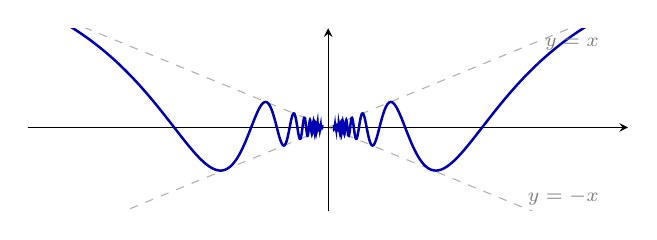
\begin{tikzpicture}
    \begin{axis}[width=9.2cm, height=3.9cm, axis lines=middle,
      xmin=-0.62, xmax=0.62, ymin=-0.42, ymax=0.5,
      xtick=\empty, ytick=\empty, clip=true]
      \addplot[gray!60, dashed, domain=-0.6:0.6, samples=2] {x};
      \addplot[gray!60, dashed, domain=-0.6:0.6, samples=2] {-x};
      \addplot[blue!70!black, line width=0.9pt, domain=0.012:0.6,
        samples=900] {x*sin(deg(1/x))};
      \addplot[blue!70!black, line width=0.9pt, domain=-0.6:-0.012,
        samples=900] {x*sin(deg(1/x))};
      \node[gray, anchor=east] at (axis cs:0.58,0.42) {\scriptsize $y=x$};
      \node[gray, anchor=east] at (axis cs:0.58,-0.35) {\scriptsize $y=-x$};
    \end{axis}
  \end{tikzpicture}
  \end{center}

  \note{
    Our first example is the function defined in equation 7: "x" times sine
    of one over "x" for nonzero "x", and zero at "x" equals zero. The plot
    shows what it looks like. As "x" approaches zero, one over "x" blows
    up, so the sine oscillates faster and faster; but the factor "x"
    squeezes the wiggles between the two dashed lines, "y" equals "x" and
    "y" equals minus "x". That squeezing is exactly why the function is
    continuous at zero, as we saw back in Chapter 4. The question now is:
    is it differentiable at zero? For the moment we take for granted that
    the derivative of sine is cosine; trigonometric functions are treated
    properly in Chapter 8. First, the easy part: away from zero.
  }
\end{frame}

% --- Build 2/3 ---
\begin{frame}{Example 5.6(a): $x \sin(1/x)$}
  \begin{exblock}{Away from $0$: Theorems 5.3 and 5.5 apply}
    \begin{equation}
      f'(x) = \sin\frac{1}{x} - \frac{1}{x}\cos\frac{1}{x}
      \qquad (x \neq 0) \tag{8}
    \end{equation}
  \end{exblock}

  \begin{hlbox}
  \textbf{Note:} at $x = 0$ these theorems say nothing --- $1/x$ is not even
  defined.
  \end{hlbox}

  \note{
    For "x" different from zero, the function is built from pieces we can
    handle: a product of "x" with a composition of sine and one over "x".
    So the product rule and the chain rule apply, and a short computation
    gives equation 8 for the derivative. Notice the second term: one over
    "x" times cosine of one over "x". It comes from the chain rule, the
    inner derivative of one over "x" being minus one over "x" squared. But
    be careful: at "x" equals zero these theorems are silent, since one
    over "x" does not exist there. To decide differentiability at zero we
    must go back to the definition.
  }
\end{frame}

% --- Build 3/3 ---
\begin{frame}{Example 5.6(a): $x \sin(1/x)$}
  \begin{exblock}{At $x = 0$: back to the definition}
    For $t \neq 0$:
    \[
      \frac{f(t) - f(0)}{t - 0} = \sin\frac{1}{t}
    \]
    As $t \to 0$ this oscillates between $-1$ and $1$ ---
    \alert{no limit exists}.
  \end{exblock}

  \vspace{0.5em}
  \hl{$\Rightarrow$ $f$ is continuous at $0$, but $\boxed{f'(0) \text{ does
  not exist}}$}

  \note{
    At zero we compute the difference quotient directly. Since "f" of zero
    is zero, the quotient is "f" of "t" over "t", and the factor "t"
    cancels, leaving just sine of one over "t". As "t" tends to zero, this
    oscillates between minus one and plus one forever, so the limit does
    not exist, and "f" prime of zero does not exist. The moral: the
    function is continuous at zero, yet the secant slopes refuse to settle
    down. Now, can we damp the oscillation enough to get a derivative?
    Yes, with one more factor of "x".
  }
\end{frame}

% --- Build 1/4 ---
\begin{frame}{Example 5.6(b): $x^2 \sin(1/x)$}
  \begin{exblock}{Example 5.6(b)}
    \begin{equation}
      f(x) = \begin{cases} x^2 \sin \dfrac{1}{x} & (x \neq 0), \\[4pt]
        0 & (x = 0). \end{cases} \tag{9}
    \end{equation}
  \end{exblock}

  \begin{center}
  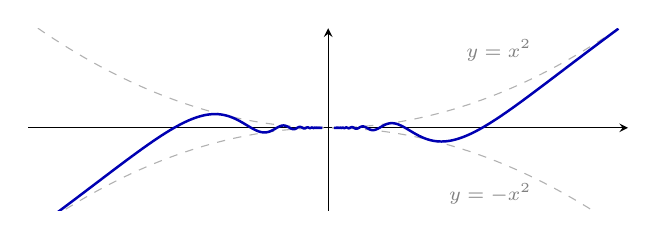
\begin{tikzpicture}
    \begin{axis}[width=9.2cm, height=3.9cm, axis lines=middle,
      xmin=-0.62, xmax=0.62, ymin=-0.3, ymax=0.36,
      xtick=\empty, ytick=\empty, clip=true]
      \addplot[gray!60, dashed, domain=-0.6:0.6, samples=120] {x^2};
      \addplot[gray!60, dashed, domain=-0.6:0.6, samples=120] {-x^2};
      \addplot[blue!70!black, line width=0.9pt, domain=0.012:0.6,
        samples=900] {x^2*sin(deg(1/x))};
      \addplot[blue!70!black, line width=0.9pt, domain=-0.6:-0.012,
        samples=900] {x^2*sin(deg(1/x))};
      \node[gray, anchor=east] at (axis cs:0.44,0.28) {\scriptsize $y=x^2$};
      \node[gray, anchor=east] at (axis cs:0.44,-0.24) {\scriptsize $y=-x^2$};
    \end{axis}
  \end{tikzpicture}
  \end{center}

  \note{
    Example "b" replaces the factor "x" by "x" squared: equation 9 defines
    "f" of "x" as "x" squared times sine of one over "x" for nonzero "x",
    and zero at zero. Look at the plot. The oscillation near zero is the
    same, infinitely many wiggles, but now the envelope is the pair of
    dashed parabolas, "y" equals "x" squared and "y" equals minus "x"
    squared. These parabolas flatten out at the origin, and that flatness
    is what will tame the secant slopes. Let's redo both computations for
    this function.
  }
\end{frame}

% --- Build 2/4 ---
\begin{frame}{Example 5.6(b): $x^2 \sin(1/x)$}
  \begin{exblock}{Away from $0$: as before, Theorems 5.3 and 5.5 give}
    \begin{equation}
      f'(x) = 2x\sin\frac{1}{x} - \cos\frac{1}{x} \qquad (x \neq 0) \tag{10}
    \end{equation}
  \end{exblock}

  \note{
    Away from zero, the product rule and chain rule again do all the work,
    and we get equation 10: the derivative is two "x" times sine of one
    over "x", minus cosine of one over "x". Keep your eye on that second
    term, the bare cosine of one over "x" with no damping factor in front.
    It is about to become the star of the show. But first, what happens at
    zero?
  }
\end{frame}

% --- Build 3/4 ---
\begin{frame}{Example 5.6(b): $x^2 \sin(1/x)$}
  \begin{exblock}{Away from $0$: as before, Theorems 5.3 and 5.5 give}
    \begin{equation}
      f'(x) = 2x\sin\frac{1}{x} - \cos\frac{1}{x} \qquad (x \neq 0) \tag{10}
    \end{equation}
  \end{exblock}

  \begin{exblock}{At $x = 0$: the definition, plus a squeeze}
    \[
      \left|\frac{f(t) - f(0)}{t - 0}\right| = \left|t \sin\frac{1}{t}\right|
      \leq |t| \qquad (t \neq 0)
      \quad\Longrightarrow\quad
      f'(0) = 0 \tag{11}
    \]
  \end{exblock}

  \note{
    At zero, we again go back to the definition. The difference quotient is
    now "t" squared times sine of one over "t", divided by "t", which is
    "t" times sine of one over "t". Its absolute value is at most the
    absolute value of "t", since sine is bounded by one; that is the
    inequality on the slide. Letting "t" tend to zero, the quotient is
    squeezed to zero, so by equation 11 the derivative at zero exists and
    equals zero. The extra factor of "t", inherited from the "x" squared,
    is precisely what example "a" was missing. So this function is
    differentiable at every point of the real line. And yet something is
    wrong with its derivative.
  }
\end{frame}

% --- Build 4/4 ---
\begin{frame}{Example 5.6(b): $x^2 \sin(1/x)$}
  \begin{exblock}{Away from $0$: as before, Theorems 5.3 and 5.5 give}
    \begin{equation}
      f'(x) = 2x\sin\frac{1}{x} - \cos\frac{1}{x} \qquad (x \neq 0) \tag{10}
    \end{equation}
  \end{exblock}

  \begin{exblock}{At $x = 0$: the definition, plus a squeeze}
    \[
      \left|\frac{f(t) - f(0)}{t - 0}\right| = \left|t \sin\frac{1}{t}\right|
      \leq |t| \qquad (t \neq 0)
      \quad\Longrightarrow\quad
      f'(0) = 0 \tag{11}
    \]
  \end{exblock}

  \begin{hlbox}
  \textbf{Punch line:} $f$ is differentiable \alert{everywhere}, but $f'$ is
  \alert{not continuous} at $0$ --- the term $\cos(1/x)$ in (10) has no limit
  as $x \to 0$.
  \end{hlbox}

  \note{
    Here is the punch line, and it is a famous one. The function is
    differentiable at every single point: equation 10 handles the nonzero
    points, and equation 11 handles zero. But look at the derivative as a
    function. As "x" tends to zero, the first term of equation 10 tends to
    zero, while the cosine of one over "x" term oscillates between minus
    one and one without any limit. So "f" prime has no limit at zero, even
    though "f" prime of zero exists and equals zero. In other words, a
    derivative can exist everywhere and still fail to be continuous.
    Derivatives are not as well behaved as one might hope, and later in
    this chapter we will discover what special properties they do have.
    Let's summarize.
  }
\end{frame}
}

{
\usebackgroundtemplate{%
  
\includegraphics[width=\paperwidth,height=\paperheight,keepaspectratio=false]{chapter_05_bg_07.png}%
}
\section{Summary}

% --- Build 1/3 ---
\begin{frame}{Summary}
  \begin{hlbox}
  \textbf{Key takeaways from this section:}
  \begin{itemize}
    \item \textcolor{defcolor}{\textbf{Definition 5.1:}} $f'(x)$ is the limit
      of difference quotients --- the slope of the tangent line
  \end{itemize}
  \end{hlbox}

  \note{
    Let's review what we covered. The derivative, Definition 5.1, is the
    limit of the difference quotients, the slopes of secant lines through
    the graph. When that limit exists, its value is the slope of the
    tangent line at the point, and "f" prime becomes a new function whose
    domain is the set of points where the limit exists. Next, the theorems.
  }
\end{frame}

% --- Build 2/3 ---
\begin{frame}{Summary}
  \begin{hlbox}
  \textbf{Key takeaways from this section:}
  \begin{itemize}
    \item \textcolor{defcolor}{\textbf{Definition 5.1:}} $f'(x)$ is the limit
      of difference quotients --- the slope of the tangent line
    \item \textcolor{thmcolor}{\textbf{Theorems 5.2, 5.3, 5.5:}}
      differentiable $\Rightarrow$ continuous; sum, product, quotient rules;
      the chain rule $h'(x) = g'(f(x))f'(x)$
  \end{itemize}
  \end{hlbox}

  \note{
    We proved three theorems. Theorem 5.2: differentiability at a point
    implies continuity there, by the quotient times increment trick.
    Theorem 5.3: sums, products, and quotients of differentiable functions
    are differentiable, with the familiar formulas, so polynomials and
    rational functions are differentiable. And Theorem 5.5, the chain rule:
    the derivative of a composition is the product of the derivatives, with
    the outer derivative evaluated at the inner value. Its proof introduced
    the powerful idea of linearization with vanishing error terms. And
    finally, the examples.
  }
\end{frame}

% --- Build 3/3 ---
\begin{frame}{Summary}
  \begin{hlbox}
  \textbf{Key takeaways from this section:}
  \begin{itemize}
    \item \textcolor{defcolor}{\textbf{Definition 5.1:}} $f'(x)$ is the limit
      of difference quotients --- the slope of the tangent line
    \item \textcolor{thmcolor}{\textbf{Theorems 5.2, 5.3, 5.5:}}
      differentiable $\Rightarrow$ continuous; sum, product, quotient rules;
      the chain rule $h'(x) = g'(f(x))f'(x)$
    \item \textcolor{excolor}{\textbf{Examples 5.6:}} continuity
      $\not\Rightarrow$ differentiability; a derivative can exist everywhere
      yet be \alert{discontinuous}
  \end{itemize}

  \vspace{0.6em}
  \textbf{Coming up next:} Mean Value Theorems --- how the derivative
  controls the global behavior of $f$.
  \end{hlbox}

  \note{
    Finally, the examples taught us humility. The function "x" sine of one
    over "x" is continuous at zero but not differentiable there, and "x"
    squared sine of one over "x" is differentiable everywhere yet has a
    discontinuous derivative. So the implication of Theorem 5.2 cannot be
    reversed, and derivatives need not be continuous. In the next section
    we prove the mean value theorems, which connect the derivative at
    interior points to the overall change of the function across an
    interval, and which are the true workhorses of differential calculus.
    See you there.
  }
\end{frame}
}

\end{document}
